% =====================================================================
%  MT-Esra — Three-Phase Compilation (one dense page per phase)
%  Knowledge-Guided RL for Building Automation
%  Stack: JaCaMo (Jason BDI + CArtAgO) - tabular Q-learning - KG/stereotypes - Node-RED
%  Compile with pdfLaTeX.
% =====================================================================
\documentclass[10pt,a4paper]{article}

\usepackage[T1]{fontenc}
\usepackage[utf8]{inputenc}
\usepackage[a4paper,margin=0.6in]{geometry}
\usepackage{amsmath,amssymb}
\usepackage{booktabs}
\usepackage{array}
\usepackage[table]{xcolor}
\usepackage{enumitem}
\usepackage{caption}
\usepackage{tikz}
\usetikzlibrary{arrows.meta,positioning,fit,backgrounds}

% ---- compact layout -------------------------------------------------
\usepackage{titlesec}
\titlespacing*{\section}{0pt}{4pt}{2pt}
\titlespacing*{\subsection}{0pt}{3pt}{1pt}
\titleformat{\section}{\normalfont\large\bfseries\color{black!85}}{\thesection.}{0.4em}{}
\titleformat{\subsection}{\normalfont\bfseries}{}{0em}{}
\setlist{nosep,leftmargin=1.2em,topsep=1pt}
\setlength{\parindent}{0pt}
\setlength{\parskip}{1.5pt}
\captionsetup{font=footnotesize,skip=2pt}
\renewcommand{\arraystretch}{1.05}

% ---- helpers --------------------------------------------------------
\newcommand{\file}[1]{\texttt{\small #1}}
\newcommand{\kw}[1]{\textbf{#1}}
\definecolor{kgblue}{RGB}{20,80,150}
\definecolor{boxgrey}{RGB}{240,240,244}
\providecommand{\checkmark}{\ensuremath{\surd}}
\newcommand{\good}{\textcolor{green!55!black}{\checkmark}}
\newcommand{\headrow}[1]{\rowcolor{boxgrey}#1}

\tikzset{
  pbox/.style={draw,rounded corners=2pt,fill=boxgrey,inner sep=3pt,
               font=\scriptsize\sffamily,align=center,minimum height=8mm},
  flow/.style={-{Stealth[length=2mm]},thick,kgblue}
}

\pagestyle{empty}

\begin{document}

% ---- provenance banner (2026-07-19) ---------------------------------
\noindent\fbox{\parbox{\dimexpr\linewidth-2\fboxsep-2\fboxrule}{\footnotesize
\textbf{PROVENANCE — historical record (pre-inversion, superseded).} Every run ID and
number in this compilation predates the action-space inversion of 2026-07-10
(\file{docs/ACTION\_SPACE\_INVERSION.md}) and, for lab3, uses spill physics that was
retuned on 2026-07-08 (original $+50$\,lux\,/\,$0.25$\,Sun and bumped
$+150$\,lux\,/\,$0.40$\,Sun; current: $+100$\,lux\,/\,$0.30$\,Sun). Quote nothing here as
current evidence: the post-inversion runs of record are listed in
\file{docs/\_audit/THESIS\_STATE\_REPORT.md} §9.1 (Phase-1 headline: arm-C run
\texttt{29639767776}, measured with \texttt{cross\_zone\_bonus = 0}).}}
\vspace{4pt}

% =====================================================================
%  PHASE 1
% =====================================================================
\begin{center}
  {\Large\bfseries Phase 1 — The Clean Ladder}\\[1pt]
  {\footnotesize \emph{Does priming a Q-learner with the Knowledge Graph (KG) make it converge
  faster than a tabula-rasa learner on clean problems with no hidden traps?}}
\end{center}
\vspace{-2pt}

\section{Labs}
Three \kw{strictly clean} labs: simulator physics is fully KG-aligned, so every
\(\textsf{ql\_true}-\textsf{ql\_false}\) difference is attributable to the prior. Each loads only
its own self-contained \file{building\_*.ttl}; the ladder adds exactly one mechanism class per step.
Discretisation (agent sees rank 0--3, never raw lux): light bounds \([50,100,300]\), sun \([50,200,600]\);
ambient \(25\) lux; horizon \(20\) steps; sun \(\in\{0,100,400,900\}\) pinned per episode (\(P(\text{sun}\!\ge\!1)=0.75\)).

\begin{center}\footnotesize
\begin{tabular}{@{}llp{6.9cm}rl@{}}
\toprule
\rowcolor{boxgrey} Lab & Port & New mechanism / physics & States & \(\langle\)eps,\,\(\varepsilon\)-dec\(\rangle\)\\
\midrule
\file{lab1} & 1892 & 1 zone, 1 \kw{Causes} lamp. \(Z1=25+0.10\,\text{Sun}+(\text{Light}?400)\); sun a pure distractor & 8 & 1000, .9920\\
\file{lab2} & 1893 & 2 \emph{independent} zones, lamp \kw{Causes} \,+\, blind \kw{Mediates}(sun). \(\text{Lvl}=25+(\text{Light}?400)+(\text{Blind}?0.5\,\text{Sun})\) & 1024 & 2000, .9960\\
\file{lab3} & 1894 & + cross-zone spill (then +50 lux / \(0.25\,\text{Sun}\); retuned 2026-07-08 to +100 / \(0.30\,\text{Sun}\)) + shared \kw{spotlight} trap (+150, never enough alone) & 2048 & 3000, .9970\\
\bottomrule
\end{tabular}
\end{center}

\vspace{-2pt}
\begin{center}
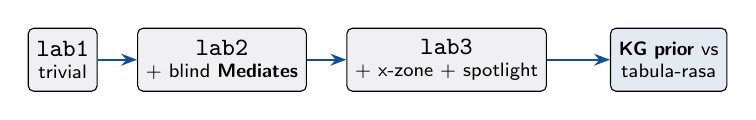
\begin{tikzpicture}[node distance=5mm]
  \node[pbox] (l1) {\file{lab1}\\trivial};
  \node[pbox,right=of l1] (l2) {\file{lab2}\\+ blind \kw{Mediates}};
  \node[pbox,right=of l2] (l3) {\file{lab3}\\+ x-zone + spotlight};
  \node[pbox,right=8mm of l3,fill=kgblue!12] (q) {\textbf{KG prior} vs\\tabula-rasa};
  \draw[flow] (l1)--(l2); \draw[flow] (l2)--(l3); \draw[flow] (l3)--(q);
\end{tikzpicture}
\end{center}

\section{Agents}
Three control modes compared in every lab: \file{rule\_based} (hand-written reference, non-learning),
\file{ql\_false} (tabula-rasa Q-learning = control arm), \file{ql\_true} (same learner + KG stereotype
priors = treatment arm). BDI agents: \file{illuminance\_controller\_agent.asl} (rule-based),
\file{\_ql.asl} (training, Gradle \file{taskQl}), \file{\_bench.asl} (held-out benchmark, \file{taskBench}),
registry \file{lab\_profiles.asl}. CArtAgO artifacts: \file{QLearner.java}, \file{StereotypeReasoner.java}
(KG\(\to\)priors), \file{LabEnvironment.java}, \file{BenchmarkLogger.java}, \file{StereotypeLearner.java}.

\section{Q-learning mechanism}
\kw{Decomposed per-zone tabular Q} with a \kw{VDN joint bootstrap} target (\file{QLearner.calculateQ}).
One shared action \(a^\star=\arg\max_{a'}\sum_\zeta Q_\zeta[s',a']\) (\file{jointArgmaxAction}) is committed
by all zones, then for each zone \(z\):
\[
Q_z[s,a]\;\mathrel{+}=\;\alpha\Big(\tfrac{1}{N_z}\,\underbrace{\mathrm{clip}_{\pm50}(r_z)}_{\text{reward}}
+\;\gamma\,Q_z[s',a^\star]-Q_z[s,a]\Big),\qquad \alpha=0.1,\ \gamma=0.9 .
\]
Per-zone reward \(r_z\): step \(-1\); gap-progress \(\pm40\cdot\Delta\text{rank}\); terminal \(+200\) at the
goal-crossing edge (\(+5\)/step held); lost-goal \(-200\); no-effect \(-10\); stagnation \(-5\). Selection is
\(\varepsilon\)-greedy (\(\varepsilon:0.3\!\to\!0.01\)) over
\(\textsf{combinedQ}(s,a)=\sum_z Q_z[s,a]+\textsf{effectivePrior}(a)\), with
\(\textsf{effectivePrior}=\textsf{priorWeight}\cdot\textsf{priors}[a]\cdot\textsf{calMul}\cdot\textsf{cellMul}\).
\kw{KG prior} (\file{StereotypeReasoner}): \kw{Causes} actuators get an optimistic Q-init bonus
(\(\textsf{INIT\_BONUS}=15\)) when activation closes the gap; \kw{Mediates} blinds are instrumental-variable
(IV) gated on sun; redundant / IV-unsat actions are penalised. Three extensions are wired in: \kw{E1}
multi-seed bootstrap CIs, \kw{E2} optional PBRS shaping \(F_z=\gamma\Phi(s')-\Phi(s),\ \Phi_z=-|{\rm lvl}_z-{\rm tgt}_z|\),
\kw{E3} adaptive trust (\(\textsf{calMul}\)). Audit fixes: default \(\textsf{STEREO\_PRIOR\_SCALE}=1.0\),
\(\textsf{PRIOR\_DECAY\_FLOOR}=0.0\), bench-time prior collapse closed (\(\textsf{currentEpisodeNum}=\textsf{priorDecayEpisodes}\)
on \file{loadQTable}), \(\textsf{visitCounts}\)/trust persisted via sidecars.

\section{Final run \& results}
\kw{Headline clean contrast} \file{phase1\_kg\_only} (KG-only vs tabula-rasa, PBRS \emph{off} both arms):
GitHub Actions run \texttt{27336756264}, commit \texttt{55c0106}, paired \(n{=}10\) seeds 1--10.
Outputs: \file{analysis/out/summary\_table\_ci.csv}, \file{paired\_tests.csv}, \file{learning\_speed\_tests.csv};
per-lab roots \file{benchmark\_results\_ql\_\{true,false\}.csv}, \file{first\_goal\_stereotypes\_*.csv},
\file{coverage\_stereotypes\_*.csv}, \file{iv\_stats\_stereotypes\_*.json}, \file{bench\_step\_log\_*.csv}.

\begin{center}\footnotesize
\begin{tabular}{@{}llrrl@{}}
\toprule
\rowcolor{boxgrey} Lab & Key metric (\(\Delta=\textsf{ql\_true}-\textsf{ql\_false}\)) & \(\Delta\) & \(q_{\rm BH}\) & Verdict\\
\midrule
\file{lab1} & auc\_goal / first-goal & \(0\) / \(-11.3\)ep & ns & \kw{Null} (saturated floor — expected)\\
\midrule
\file{lab2} & auc\_goal (primary, \(\uparrow\)) & \(+0.0171\) & \(0.000\) & \good\ \(\delta=1.0\) every seed\\
\file{lab2} & mean\_first\_goal (\(\downarrow\)) & \(-32\)ep & sig & \good\ reaches goal sooner\\
\file{lab2} & avg\_redundant (\(\downarrow\)) & \(2.70\!\to\!1.49\) & sig & \good\ \(\sim45\%\) fewer\\
\file{lab2} & goal\_rate (\(\uparrow\)) & \(0.963\!\to\!1.000\) & \(0.0065\) & \good\ \kw{anchor confirmed}\\
\midrule
\file{lab3} & mean\_first\_goal (\(\downarrow\)) & \(+42.6\)ep & \(0.002\) & \(\times\) KG-alone over-explores\\
\file{lab3} & goal\_rate & \(0.994\) vs \(0.988\) & ns & tied (ceiling)\\
\file{lab3} & auc\_reward (\(\uparrow\)) & \(+16\) & sig & \good\ only robust win\\
\bottomrule
\end{tabular}
\end{center}

\kw{lab3 cross-zone refinement.} The bare optimistic prior over-explores 2048 states, so lab3 was
re-modelled with a \kw{SECONDARY (WeakOpticalCoupling)} cross-zone stereotype (KG declares the spill
\emph{structure}; RL learns the magnitude) + a gated Part-B exploration bonus, on bumped lab3 physics
(lamp \(+150\), blind \(0.40\,\text{Sun}\)). Runs \texttt{27461188614} (seeds 1--10) and replication
\texttt{27462446044} (seeds 11--20): lab3 \kw{auc\_reward} \(+14.26\) then \(+18.85\), \(\delta=+1.00\)
on \emph{every} seed in both batches; final-policy economy directional but ceiling-bound (ns).
Mechanism ablation \texttt{27464846574}: \kw{targeted} \(+14.26\,(\delta{=}1.0)\) vs \kw{untargeted}
\(+9.16\,(\delta{=}0.58)\) — the value comes from \emph{knowing where the spill goes}.
Data: \file{phase1\_xzone\_bumped\{,\_s11\_20,\_ablation\}/analysis/out/}.

\section{Analysis}
The thesis anchor — \emph{a physics-primed learner converges faster with fewer redundant actions at
equal/better success in a clean lab} — is confirmed \kw{cleanly and repeatedly on lab2} with the KG
isolated (PBRS off). \file{lab1} is the expected saturated floor. \file{lab3} is an \kw{honest scope
limit}: a bare optimistic prior cannot accelerate first-goal on a 2048-state space, but its
\kw{learning-trajectory reward (auc\_reward) is robustly higher}, and the cross-zone ablation proves the
benefit is structural targeting, not generic optimism. Negative control \file{phase1\_baseline}
(KG zeroed) returns \(\textsf{ql\_true}\approx\textsf{ql\_false}\) everywhere, \kw{securing causal attribution} to the KG.

\clearpage
% =====================================================================
%  PHASE 2
% =====================================================================
\begin{center}
  {\Large\bfseries Phase 2 — The Faulty Ladder}\\[1pt]
  {\footnotesize \emph{When a real actuator silently breaks, can the agent detect it, blacklist it,
  alert the user, and re-learn over what survives — and does the KG-primed arm recover faster?}}
\end{center}
\vspace{-2pt}

\section{Labs}
Nine \kw{faulty} profiles, each forking a clean Phase-1 parent. The \kw{KG is unchanged} (it still
believes the \emph{nominal} physics); the \kw{simulator injects exactly one hardware fault} into a
\kw{Causes} lamp. \file{adapt\_source/2} maps each faulty profile to its parent's clean Q-table, so the
adapt agent \kw{warm-loads the Phase-1 final policy} and measures \emph{recovery from a working policy}.

\begin{center}\footnotesize
\begin{tabular}{@{}lllp{6.6cm}@{}}
\toprule
\rowcolor{boxgrey} Profile & Port & Fault & Survivor structure / role\\
\midrule
\file{lab1\_f1dead} & 1892 & 1 lamp dead & \kw{Detection-only}: lone actuator, no lever survives \(\Rightarrow\) recovery N/A\\
\file{lab2\_f1dead/f1inv} & 1893 & 1 lamp dead / inverted & Z1 blind + all Z2 survive \(\Rightarrow\) recovery on sunny eps\\
\file{lab2\_f2dead/f2inv} & 1893 & both lamps dead / inverted & only sun-gated blinds survive (partial / iterative)\\
\file{lab3\_f1dead/f1inv} & 1894 & 1 lamp dead / inverted & spotlight + spill keep Z1 partly lit (cleanest inversion case)\\
\file{lab3\_f2dead/f2inv} & 1894 & both lamps dead / inverted & spotlight (+150 both) + blinds survive (cleanest several-dead recovery)\\
\bottomrule
\end{tabular}
\end{center}
Fault model: \emph{dead} = lamp lux forced \(0\) (flag still toggles, lux contribution zeroed);
\emph{inverted} = lux negated. lab3 faults train \(\langle4000,.9970\rangle\). Blinds (\kw{Mediates}) are
never injected nor adjudicated — a healthy blind looks ``dead'' at sun~0.

\section{Agents}
\kw{Strict separation preserved} — the Phase-1 learning path is byte-for-byte untouched. New BDI agent
\file{illuminance\_controller\_agent\_adapt.asl} orchestrates the lifecycle in one loop
(\file{task\_adapt.jcm}, Gradle \file{taskAdapt}). Supporting: \file{run\_phase2\_adapt.ps1} orchestrator,
\file{generate\_faulty\_flows.ps1} (9 Node-RED flows), \file{system\_prop\_num.java}. All fault logic is
additive \file{@OPERATION}s on \file{QLearner.java}.

\begin{center}
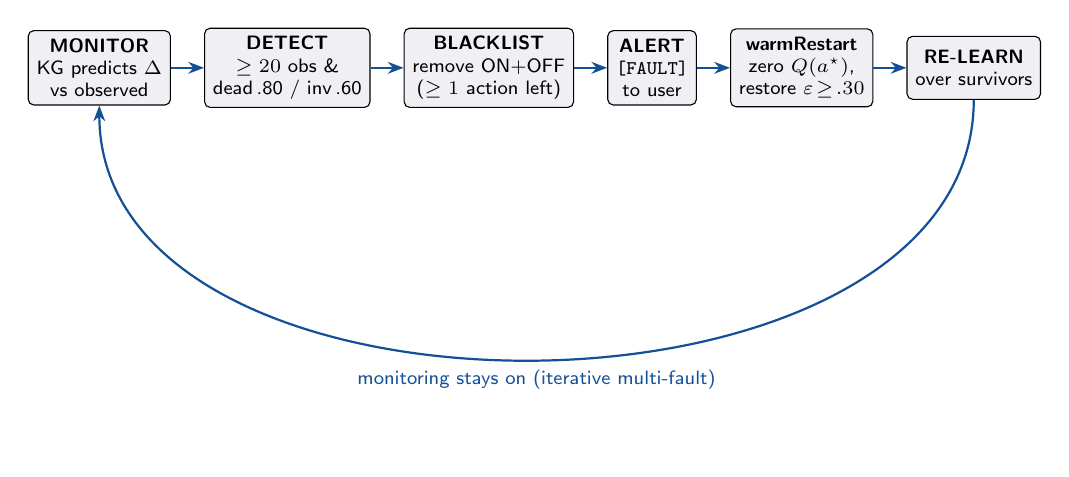
\begin{tikzpicture}[node distance=4.2mm]
  \node[pbox] (a) {\textbf{MONITOR}\\KG predicts \(\Delta\)\\vs observed};
  \node[pbox,right=of a] (b) {\textbf{DETECT}\\\(\ge20\) obs \&\\dead\,.80 / inv\,.60};
  \node[pbox,right=of b] (c) {\textbf{BLACKLIST}\\remove ON+OFF\\(\(\ge1\) action left)};
  \node[pbox,right=of c] (d) {\textbf{ALERT}\\\texttt{[FAULT]}\\to user};
  \node[pbox,right=of d] (e) {\textbf{warmRestart}\\zero \(Q(a^\star)\),\\restore \(\varepsilon\!\ge\!.30\)};
  \node[pbox,right=of e] (f) {\textbf{RE-LEARN}\\over survivors};
  \draw[flow] (a)--(b);\draw[flow] (b)--(c);\draw[flow] (c)--(d);\draw[flow] (d)--(e);\draw[flow] (e)--(f);
  \draw[flow] (f.south) to[out=-90,in=-90] node[below,font=\scriptsize\sffamily]{monitoring stays on (iterative multi-fault)} (a.south);
\end{tikzpicture}
\end{center}

\section{Q-learning mechanism (additive fault ops)}
\file{observeForFaults} reuses \file{reasoner.getActionPrediction} (expected \(\pm1\) per zone),
compares to the observed \(\Delta\), and buckets each falsifiable observation as healthy / dead / inverted —
\kw{pure accumulation, no policy mutation}. IV-gated (\kw{Mediates}) components are skipped, so only
\kw{Causes} lamps/spotlight are adjudicated (kills the prior false positive on \file{SetZ2Blinds}).
Thresholds: \(\textsf{MIN\_SAMPLES}=20,\ \textsf{DEAD}=0.80,\ \textsf{INV}=0.60,\ \textsf{ANOMALY}=0.75,\ \textsf{EPS\_BOOST}=0.30\).
\file{blacklistComponent} removes both ON+OFF indices (never \textsc{do\_nothing}); both
\file{computeApplicableActions} and the VDN \file{jointArgmaxAction} target filter blacklisted actions, so a
dead actuator can never poison \(\max_a Q\). \file{warmRestart} zeroes \(Q\)/visits of blacklisted actions,
decays poisoned states, and restores the \(\varepsilon\) floor; the KG re-primes automatically over the
filtered set. \kw{Recovery criterion} (v2.1 instrument fix) is \kw{policy-stability}: the greedy joint-argmax
policy is snapshotted each adapt episode and declared recovered after \(\textsf{RECOVERY\_WINDOW}=50\)
consecutive unchanged episodes — robust to \(\varepsilon\) and to sun-stochastic reachability (the original
Bellman-stability test gave 0\% reconvergence). v2.2 adds a greedy (\(\varepsilon{=}0\)) \(K{=}20\) rollout
certifying \(\textsf{RecoveredGoalRate}\); \kw{goal-reaching} \(\equiv\) reconverged \(\wedge\ \text{gr}\ge0.5\).
Headline: \(\textsf{RecoveryEpisodes}=\textsf{ReconvergeEpisode}-\textsf{DetectEpisode}\).

\section{Final run \& results}
Confirmatory \(n{=}10\): 9 profiles \(\times\) 2 arms \(\times\) 10 seeds \(=\) \kw{180 adapt runs} (warm-started),
GitHub Actions run \texttt{27529585379} (commit \texttt{2aab559}). Per-cell outputs
\file{recovery\_stereotypes\_\{true,false\}\_<lab>\_<fault>.csv} (columns
\texttt{DefectComponent, DetectEpisode, ReconvergeEpisode, RecoveryEpisodes, SecondaryDetectEpisode, RecoveredGoalRate}),
plus \file{qtable\_adapted\_*}, \file{metrics\_adapted\_*}; raw tree
\file{phase2\_results\_v5/recovery\_root/seed\{1..10\}/}; aggregation \file{analysis/phase2\_recovery.py}.

\begin{center}\footnotesize
\begin{tabular}{@{}lp{8.6cm}@{}}
\toprule
\rowcolor{boxgrey} Result & Finding (paired \(\textsf{ql\_true}-\textsf{ql\_false}\), BH-FDR, \(n=10\))\\
\midrule
\kw{Detection recall} & \kw{100\%} in all 18 cells; correct \texttt{DefectComponent}; attribution 17/18 (only \file{lab3\_f2inv} \textsf{ql\_true} spotlight FP). \kw{No blind false positives}.\\
\kw{Headline recovery} & \file{lab3\_f1dead} (well-posed, goal-reaching gr\,\(\approx0.92\)): \(\textsf{RecoveryEpisodes}\) \kw{144.6 vs 328.7}, \(\Delta=-184.1\), CI\([-281,-87]\), Wilcoxon \(p{=}0.0039\), \(\delta=-0.85\), \(q_{\rm BH}=0.004\) — KG re-learns \(\sim2.3\times\) faster.\\
\kw{Compensation} & \file{lab3\_f1inv}: KG \emph{detects slower} \(\Delta\textsf{DetectEp}=+120.1\), \(\delta=0.99\), \(q_{\rm BH}{=}0\) — primed policy routes around a single fault, under-sampling it.\\
\kw{Futile cells} & \file{lab2\_f2*}, \file{lab3\_f2inv}: goal physically unreachable post-fault (only sun-gated blinds survive) \(\Rightarrow\) gr\,\(\approx 0.02\text{--}0.3\), correctly flagged ``stable-but-futile''.\\
\bottomrule
\end{tabular}
\end{center}

\section{Analysis}
Two capabilities are demonstrated. \kw{(1) Detection is universal and precise}: the KG's nominal-physics
monitor fires on every injected \kw{Causes} fault and the IV-gating fix means healthy blinds are never
mis-flagged. \kw{(2) The recovery benefit is complexity-gated}: KG-priming wins recovery in proportion to
\emph{exploitable survivor structure} — decisively in \file{lab3\_f1dead} (deterministic spotlight + spill
give a fixed greedy optimum), while trivial labs tie or favour rule-based, and physically-unrecoverable
multi-fault cells are correctly certified futile by the goal-rate test. The recurring
\kw{robustness\(\leftrightarrow\)diagnosability trade-off} (rich labs hide a single fault from detection,
yet the same richness powers faster re-learning) is replicated three times and is itself a thesis finding.

\clearpage
% =====================================================================
%  PHASE 3
% =====================================================================
\begin{center}
  {\Large\bfseries Phase 3 — The Slow Ladder}\\[1pt]
  {\footnotesize \emph{Can the agent learn each actuator's temporal response delay online, write it back
  to the KG, and use it to satisfy time-bounded goals (``bright now'' vs ``bright within 5 min'')?}}
\end{center}
\vspace{-2pt}

\section{Labs}
Two \kw{slow} profiles, structurally identical to their clean parents (same agent ontology, targets,
bounds \(\Rightarrow\) \kw{same Q-state space}), but the simulator gives the motorized blind a
\kw{temporal response delay} while lamps and the spotlight stay instantaneous.

\begin{center}\footnotesize
\begin{tabular}{@{}lllp{6.2cm}@{}}
\toprule
\rowcolor{boxgrey} Profile & Port & Dim & Delay model / role\\
\midrule
\file{lab2\_slow} & 1895 & 7 & forks \file{lab2}; \kw{one} blind delayed \(\sim\!60\)s; learn delay, prefer fast lamp when tight\\
\file{lab3\_slow} & 1896 & 8 & forks \file{lab3}; \kw{both} blinds delayed; richest temporal-planning case (delay + cross-zone)\\
\bottomrule
\end{tabular}
\end{center}
Ground truth: a 50\,ms env-tick increments \texttt{Tick} and integrates \texttt{EnergyCost} (exposed via the
new \file{readLabStatusTimed} op); the blind countdown is \(\textsf{blind\_delay\_ticks}=12\); at
\(\textsf{seconds\_per\_tick}=5.0\) that is \(60\)s of simulated time. The building TTLs are \emph{static} —
\(\textsf{ws:responseDelay}\) is \kw{not} asserted there; the learned write-back file is the canonical value.

\section{Agents}
\kw{Strict separation preserved} — no Phase-1/2 file is modified. New BDI agent
\file{illuminance\_controller\_agent\_dynamics.asl} (\(\sim\)500 lines) runs a four-stage cycle; it
\kw{does not Q-learn} (stereotypes are used only to populate the action space). New CArtAgO artifact
\file{DynamicsLearner.java} (numerically-stable Welford statistics + KG write-back). Wiring: Gradle
\file{taskDynamics}, workflow \file{phase3.yml}, runner \file{run\_phase3\_dynamics.ps1}.

\begin{center}
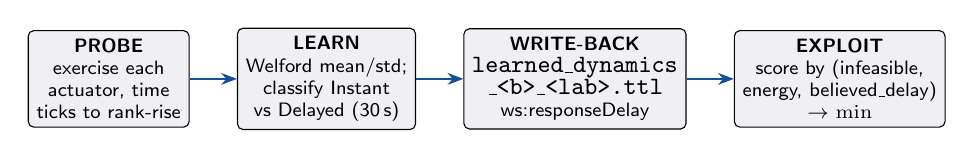
\begin{tikzpicture}[node distance=6mm]
  \node[pbox] (p) {\textbf{PROBE}\\exercise each\\actuator, time\\ticks to rank-rise};
  \node[pbox,right=of p] (l) {\textbf{LEARN}\\Welford mean/std;\\classify Instant\\vs Delayed (30\,s)};
  \node[pbox,right=of l] (w) {\textbf{WRITE-BACK}\\\file{learned\_dynamics}\\\file{\_<b>\_<lab>.ttl}\\\(\textsf{ws:responseDelay}\)};
  \node[pbox,right=of w] (e) {\textbf{EXPLOIT}\\score by (infeasible,\\energy, believed\_delay)\\\(\to\min\)};
  \draw[flow] (p)--(l);\draw[flow] (l)--(w);\draw[flow] (w)--(e);
\end{tikzpicture}
\end{center}

\section{Mechanism (temporal-dynamics learning + deadline planning)}
\kw{PROBE}: every URI-bearing actuator is exercised from a known baseline; the delay is the number of
ticks between dispatching the WoT action and the first observed rise in the controlled zone rank
(\(\textsf{probes\_per\_actuator}=8\), settle \(400\)ms, poll \(50\)ms, cap \(60\) ticks).
\kw{LEARN}: per-action Welford running mean/std over \(\textsf{delay\_ticks}\); classify
\(\textsf{InstantaneousResponse}\) if \(\text{mean}<\textsf{INSTANT\_THRESHOLD\_SEC}=30\)s (=\(6\) ticks), else
\(\textsf{DelayedResponse}\). \kw{WRITE-BACK}: emit \file{learned\_dynamics\_<bool>\_<profile>.ttl} carrying
\(\textsf{ws:responseDelay}\) (s), \(\textsf{responseDelayTicks}\), samples, std, class; reload as a
\(\textsf{learned\_delay\_sec(Action,Sec)}\) belief. \kw{EXPLOIT}: for each time-bounded goal, every action
that \emph{can} reach the target zone-rank is scored by
\((\textsf{infeasible-flag},\ \textsf{energy\_cost},\ \textsf{believed\_delay})\) and the \(\min\) is chosen.
The \kw{KG-primed} arm reads \(\textsf{believed\_delay}\) from the learned KG; the \kw{tabula-rasa} arm
believes every action is instantaneous (\(\textsf{believed\_delay}=0\)), so under a tight deadline it grabs
the cheapest (slow) actuator and misses.

\section{Final run \& results}
Confirmatory \(n{=}10\) (default \file{phase3.yml} \texttt{replicas=1..10}, 8 probes), GitHub Actions run
\texttt{27621106006}, merged to \texttt{main} via PR\,\#2 (\texttt{3bb5289}). Outputs:
\file{dynamics\_delays\_\{true,false\}\_\{lab2\_slow,lab3\_slow\}.csv}
(\texttt{action\_label, action\_value, samples, delay\_ticks, delay\_seconds, std\_ticks, response\_class}),
\file{learned\_dynamics\_\{true,false\}\_<lab>.ttl}, and a per-goal exploit CSV
(\texttt{profile, mode, goal\_id, zone, target\_rank, deadline\_sec, chosen\_label, believed\_delay\_sec,
learned\_delay\_sec, actual\_delay\_sec, energy\_cost, met}); aggregation \file{analysis/phase3\_dynamics.py}.

\begin{center}\footnotesize
\begin{tabular}{@{}lp{8.7cm}@{}}
\toprule
\rowcolor{boxgrey} Headline & Result\\
\midrule
\kw{Delay accuracy} & learned blind \kw{12.11--12.21} ticks vs ground-truth \kw{12} \(\Rightarrow\) rel.\ err \(\le1.77\%\); instant actuators \(\sim\!1.14\)t; \kw{classification 100\% correct} (\(+0.15\)t bias = first-tick-crossed + poll quantum).\\
\kw{Compliance} & 6 goals (3 \kw{tight} 15/45/15\,s, 3 \kw{loose} 90/300/300\,s): \(\textsf{ql\_true}\) \kw{6/6} (tight 1.0, loose 1.0); \(\textsf{ql\_false}\) \kw{3/6} (tight \kw{0.0}, loose 1.0). Mean actual delay \(\sim\!33\)s vs \(\sim\!60.6\)s.\\
\kw{Paired test} & \kw{tight} \(\Delta=+1.0\), CI\([1,1]\), \(p_{\rm boot}{=}0\), Cliff's \(\delta{=}1.0\), \(q_{\rm BH}{=}0\); \kw{overall} \(+0.5\), CI\([0.5,0.5]\); per-profile \(n{=}10\) \(\Rightarrow p_{\rm Wilcoxon}=2/2^{10}=0.00195\) clears 0.05.\\
\kw{Energy trade-off} & \(\textsf{ql\_true}\approx 3.2\text{--}3.3\) (lamps for tight goals) vs \(\textsf{ql\_false}=0\) (always the free slow blind) — the honest cost of compliance.\\
\bottomrule
\end{tabular}
\end{center}

\section{Analysis}
Both headlines are confirmed. The KG-primed agent \kw{learns each actuator's delay to \(\sim\!1.5\%\)},
writes it back to the KG, and \kw{plans against deadlines}: it reaches for the fast lamp on every tight
deadline while the tabula-rasa planner — believing everything instantaneous — grabs the cheap slow blind
and misses all three tight goals. Because the exploit planner is \kw{deterministic}, point estimates are
bit-identical from \(n{=}5\) to \(n{=}10\); the larger sample only clears the Wilcoxon-floor formality. An
\kw{emergent} observation: in \file{lab3\_slow}, \(\textsf{ql\_true}\) chose the \emph{other} zone's blind
for zone-1 loose goals, empirically re-discovering the Phase-1 cross-zone bleed (\(0.40\,\text{Sun}\)) from
data via \(\textsf{action\_effect/3}\) — benign and lab-specific. \kw{Phase 3 is complete}; the energy gap
is a genuine trade-off, not a regression.

\end{document}
